%!TEX root = mainShort.tex
\section{A-Graphs}
\seclabel{quad}
\seclabel{quadrangulations}

In this section, we study a special class of graphs that are closely
related to quadrangulations in which every edge crosses $Y$. (See \figref{a-graph} for an example.)

\begin{definition}\deflabel{a-graph}
	An \emph{A-graph}, $G$, is a \Fary\ embedding of a graph with $n\ge 3$ vertices that has the following properties: (1) Every edge of $G$ intersects $Y$ in exactly one point, possibly an endpoint. (2) Every face of $G$, including the outer face, is a quadrilateral or a triangle. (3) Every quadrilateral face of $G$ is non-convex. (4) Every triangular face contains one vertex in each of $Y$, $L$, and $R$. (5) Every vertex $v$ on $Y$ is incident to precisely
		two triangular faces, one ``above $v$'' whose interior contains the open line segment with endpoints $v$ and $v+(0,\epsilon)$ for some $\epsilon>0$ and one ``below $v$'' whose interior contains the open line segment with endpoints $v$ and $v-(0,\epsilon)$ for some $\epsilon >0$.
\end{definition}

\begin{wrapfigure}[11]{r}{.3\textwidth}
		\Vspace{-1mm}
		\centering
		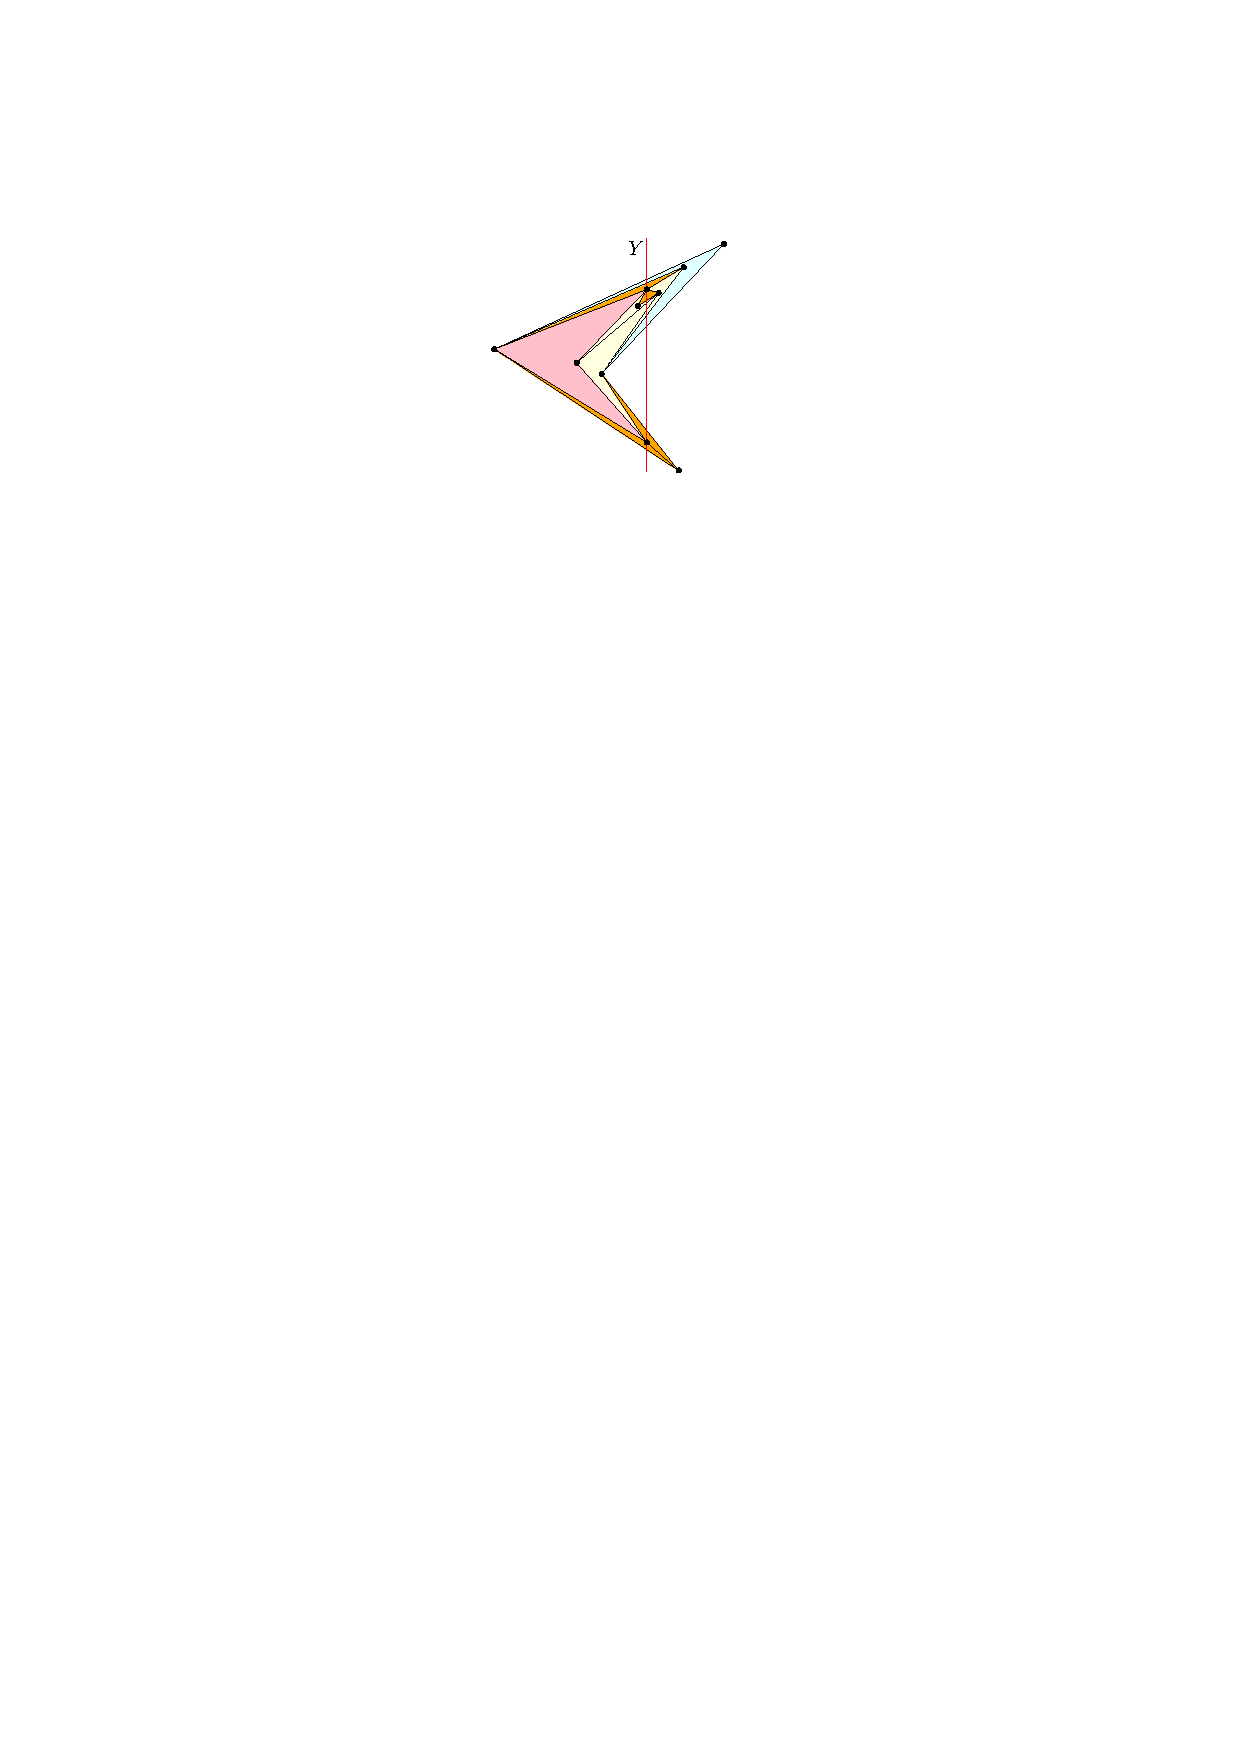
\includegraphics[scale = 0.95]{figs/a-graph-new}
		\caption{An A-graph with 2 vertices in $Y$.}
		\figlabel{a-graph}
	\end{wrapfigure}
	
In the special case where $G$ has no vertices in $Y$, the graph $G$ is a quadrangulation in which every edge crosses $Y$. Further, Property~5 applies even if $v$ is on the outer face of $G$ (in which case it implies that the outer face of $G$ must be a triangle).
Some additional properties of $G$ follow from \defref{a-graph}: (6) $G$ is connected. (7) Every vertex of $G$ has degree at least 2. (8) If $n\ge 4$, then every vertex in $Y$ has degree at least 3.  Property~6 follows directly from Property~2.
Property~7 follows from the fact that every vertex is incident to at
least one face and every face is a simple cycle.
Property~8 follows from the fact that every vertex on $Y$ is incident
to at least two triangular faces, which involve at least 4 vertices, unless $n=3$.

%We will show that every A-graph $G$ has a \Fary\ embedding with prescribed
%intersections with $Y$ and a prescribed outer face.  Since the outer
%face of an A-graph can be a triangle or a quadrilateral, in the following
%theorem, $\Delta$ is a triangle or quadrilateral defined as follows:
%\begin{enumerate}
%   \item If $(0,y_1)$ is a vertex of $G$, then $\Delta$ is a triangle
%   with one vertex at $(0,y_1)$ and the opposite edge edge crossing $Y$ at $y_m$.
%
%   \item If $(0,y_m)$ is a vertex of $G$, then $\Delta$ is a triangle
%   with one vertex at $(0,y_m)$ and the opposite edge crossing $Y$ at $y_1$.
%
%   \item Otherwise,
%      $\Delta$ is a quadrilateral whose edges cross $Y$ at $y_1$, $y_a$,
%      $y_b$, and $y_m$, where $e_1$, $e_a$, $e_b$, and $e_m$ are the four edges on the outer face of $G$
%\end{enumerate}

We will show that every A-graph $G$ has a \Fary\ embedding with prescribed intersections with $Y$ and a prescribed outer face, as in the following theorem. 

\begin{thm}\thmlabel{a-graph}
	Let $G$ be an A-graph, let $e_1,\ldots,e_m$ be the sequence of edges in $G$, in the order they are intersected by $Y$, and let $y_1\le\cdots\le y_m$ be any sequence of numbers where, for each $i\in\{1,\ldots,m-1\}$, $y_i=y_{i+1}$ if and only if $e_i$ and $e_{i+1}$ have a common endpoint in $Y$. Further, let $\Delta$ \mbox{be a triangle or quadrilateral, where:}
		\begin{compactenum}
			\item If $(0,y_1)$ is a vertex of $G$, then $\Delta$ is a triangle
			with a vertex at $(0,y_1)$ and the opposite edge crossing $Y$ at $y_m$.
			
			\item If $(0,y_m)$ is a vertex of $G$, then $\Delta$ is a triangle
			with a vertex at $(0,y_m)$ and the opposite edge crossing $Y$ at $y_1$.
			
			\item Otherwise, $\Delta$ is a quadrilateral whose edges cross $Y$ at $y_1$, $y_a$,
			$y_b$, and $y_m$, where $e_1$, $e_a$, $e_b$, and $e_m$ are the four edges on the outer face of $G$.
	\end{compactenum}
	Then $G$ has a
	\Fary\ embedding in which the outer face is $\Delta$
	and, for each $i\in\{1,\ldots,m\}$, the intersection between $e_i$ and $Y$
	is the single point $(0,y_i)$.
\end{thm}

The rest of this section is devoted to prove \thmref{a-graph}. We make some simplifying assumptions. First, we assume w.l.o.g.\ up to a uniform scaling that $\Delta$ and all the vertices of $G$ are contained in $[-1,1]^2$. Second, we assume w.l.o.g.\ up to a reflection  with respect to $Y$ that, if the outer face of $G$ is delimited by a quadrilateral, then the vertex incident to both $e_1$ and $e_m$ is in $L$, as in \figref{a-graph}. In such a case we also assume that the vertex of $\Delta$ incident to both $e_1$ and $e_m$ is in $L$; this is also not a loss of generality, as if the vertex of $\Delta$ incident to both $e_1$ and $e_m$ is in $R$, then $\Delta$ can be reflected with respect to $Y$, obtaining a quadrilateral $\Delta'$ whose vertex incident to both $e_1$ and $e_m$ is in $L$, then a \Fary\ embedding of $G$ can be constructed in which the outer face is $\Delta'$, and finally the \Fary\ embedding can be reflected with respect to $Y$, thus obtaining a \Fary\ embedding of $G$ in which the outer face is $\Delta$. 

If $m=3$ or $m=4$, then $G$ is a 3- or a 4-cycle, respectively, hence it suffices to embed it as $\Delta$. Therefore we assume, from now on, that $m\ge 5$.  

%Since the rest of this section is a proof of \thmref{a-graph}, we will
%use the notations $G$, $e_1,\ldots,e_m$, $y_1,\ldots,y_m$, and $\Delta$
%that appear in the statement of \thmref{a-graph} consistently throughout
%this section.  \thmref{a-graph} is trivial if $m=3$ since, in this
%case $G$ is a single 3-cycle that we embed as $\Delta$. Therefore we
%will assume, from this point onward, that $m\ge 4$.  Without loss of
%generality (by uniform scaling of all quantities), we will also assume
%that $\Delta\subset [-1,1]^2$.

%A vertex $v\in Y$ has its neighbours partitioned
%into two sets $\alpha_1,\ldots,\alpha_k\in L$ and
%$\beta_1,\ldots,\beta_\ell\in R$. This partitions $v$'s incident
%edges into $a_1,\ldots,a_k\in L\cup Y$ and $b_1,\ldots,b_\ell\in
%Y\cup R$.

	\begin{wrapfigure}[10]{r}{.32\textwidth}
		\Vspace{-1mm}
		\centering
		\includegraphics[scale = 0.95]{figs/ab}
		\caption{The ordering of the edges incident to a vertex $v$ on $Y$.}
		\figlabel{ab}
	\end{wrapfigure}
Before continuing, we pause to fully specify the ordering
$e_1,\ldots,e_m$. This ordering is unambiguous except where
some vertex $v\in Y$ is incident to several edges
$e_{i},\ldots,e_{i+d}$, where $d\ge 2$ by Property~8 of A-graphs. Refer to \figref{ab}.  In this case we partition $v$'s neighbors into two
sets $\alpha_1,\ldots,\alpha_k\in L$ and $\beta_1,\ldots,\beta_\ell\in
R$, where $\alpha_1,\ldots,\alpha_k$ are ordered clockwise around $v$
and $\beta_1,\ldots,\beta_\ell$ are ordered counterclockwise.  We then use
the convention that $e_i,\ldots,e_{i+k-1}=v\alpha_1,\ldots,v\alpha_k$
and $e_{i+k},\ldots,e_{i+d}=v\beta_1,\ldots,v\beta_\ell$.

We will describe the desired \Fary\ embedding by assigning a slope
$s_i$ to each edge $e_i\in E(G)$.  
Since there can be no vertical edges, $s_i$ is well-defined.
We have $m=|E(G)|$ slope variables, $s_1,\ldots,s_m$.  Since every edge
$e_i$ contains the point $(0,y_i)$, the slope $s_i$
fixes the line through $e_i$.  Since every vertex $v$ not on $Y$ is
incident to at least two edges that contain distinct points on $Y$,
the location of $v$ is fixed.  (The location of each vertex on $Y$
is fixed by definition.)

A necessary condition for the slopes to determine a F\'ary embedding of $G$ is that the supporting lines of edges 
with a common vertex should be concurrent. Let $v$ be a vertex 
not on $Y$, and let $e_i, e_j, e_k$ be three edges incident to $v$.
The fact that the supporting lines of $e_i$, $e_j$, and $e_k$
meet at a common point (the location of $v$) is expressed by the following
\emph{concurrency constraint} in terms of the slopes $s_i,s_j,s_k$:
\begin{equation}\eqlabel{slope0} 
\left|
\begin{matrix}
1&1&1\\
s_i&s_j&s_k\\
y_i&y_j&y_k
\end{matrix}
\right|=
({y_j-y_k}) s_i + ({y_k-y_i}) s_j 
+ ({y_i-y_j})s_k  = 0
\end{equation}
Since $y_1,\ldots,y_m$ are given, this is a linear equation
in $s_1,\ldots,s_m$.
Writing this equation for all triplets of edges incident to a common
vertex $v$ will include many redundant equations. Indeed, it suffices to take $d_v-2$ equations: We choose two fixed
incident edges $e_i$ and $e_j$ and run $e_k$ through the remaining
$d_v-2$ edges, specifying that $e_k$ should go through the common vertex
of $e_i$ and $e_j$.
%We call the resulting collection of $\sum_{v\in V(G)\setminus Y} d_v-2$ equations the \emph{concurrency constraints}.

Whenever convenient, we will use edges of $G$
as indices so that, if $e=e_i$ is an edge of $G$, then $s_e=s_i$
and $y_e=y_i$.  Further, if $e$ is a line segment that
intersects $Y$ in a point, we will use $y_e$ to denote the $y$-coordinate
of the intersection of $e$ and $Y$ and $s_e$ to denote the slope of
$e$'s supporting line.

%It will be important to have as many equations as variables;
%thus, 

We now introduce additional equations for the edges that emanate from a
vertex on $Y$.
Suppose that a vertex $v\in Y$ is incident to edges $a_1,\ldots,a_k\in L\cup Y$ 
and $b_1,\ldots,b_\ell\in Y\cup R$, ordered from bottom to top as in \figref{ab}.
From Property~4 of A-graphs we have $k,\ell\ge1$ and, from Property~8, we have $k+\ell\ge 3$.
We want the slopes of the edges on the right side to be increasing:
$s_{b_1} < s_{b_2} < \dots  <s_{b_\ell}$. We stipulate a stronger
condition, namely that $s_{b_2}, \dots, s_{b_{\ell-1}}$ partition the interval
$[s_{b_1},s_{b_\ell}]$ in fixed proportions. That is:
\begin{equation}
\label{eq:proportion}
s_{b_i} = s_{b_1} + \lambda_i(s_{b_{\ell}}-s_{b_1}),
\end{equation}
for some fixed sequence $0<\lambda_2<\cdots<\lambda_{\ell-1}<1$.

For example, we might set $\lambda_i := (i-1)/(l-1)$.
This gives $\ell-2$ equations, for $\ell\ge 2$. Similarly, we get
$k-2$ equations for the slopes
$s_{a_1}, \dots, s_{a_{k}}$ of the edges on the left side, for $k\ge 2$.
In addition, for $k\ge 2$ and $\ell\ge 2$, we require that the \emph{range} of
slopes
on the two sides are in a fixed proportion:
\begin{equation}
\label{eq:proportion2}
s_{a_1}-s_{a_{k}} = \mu (s_{b_{\ell}}-s_{b_1}),
\end{equation}
for some fixed value $\mu>0$.
%
We call the equations
\thetag{\ref{eq:proportion}--\ref{eq:proportion2}} the
\emph{proportionality constraints}.
There are $(k+\ell)-3$ such equations for the $k+\ell$ slopes, hence we have three degrees of freedom for the slopes out of a vertex.
%\figref{proportional} illustrates these  degrees of freedom:
Namely, we can shear the edges on the right side vertically, adding the same constant to all
slopes. We can independently shear all edges on the left side.
In addition, we can vertically scale {all} lines jointly (both to
the left and to the right), multiplying all slopes by the same constant factor.
If this factor is negative, we would reverse the order of the
slopes, simultaneously on the left and on the right. We will later see how to prevent this. We can already observe that two slopes on one side determine all remaining slopes on that side. Moreover, the range of slopes on the other side ($s_{a_1}-s_{a_{k}}$ or $s_{b_{\ell}}-s_{b_1}$) is also determined.
%
The notations $\lambda_i$ and $\mu$ are here used in a local sense;
for a different vertex $v$, we may choose different constants.
%\begin{figure}
%	\centering{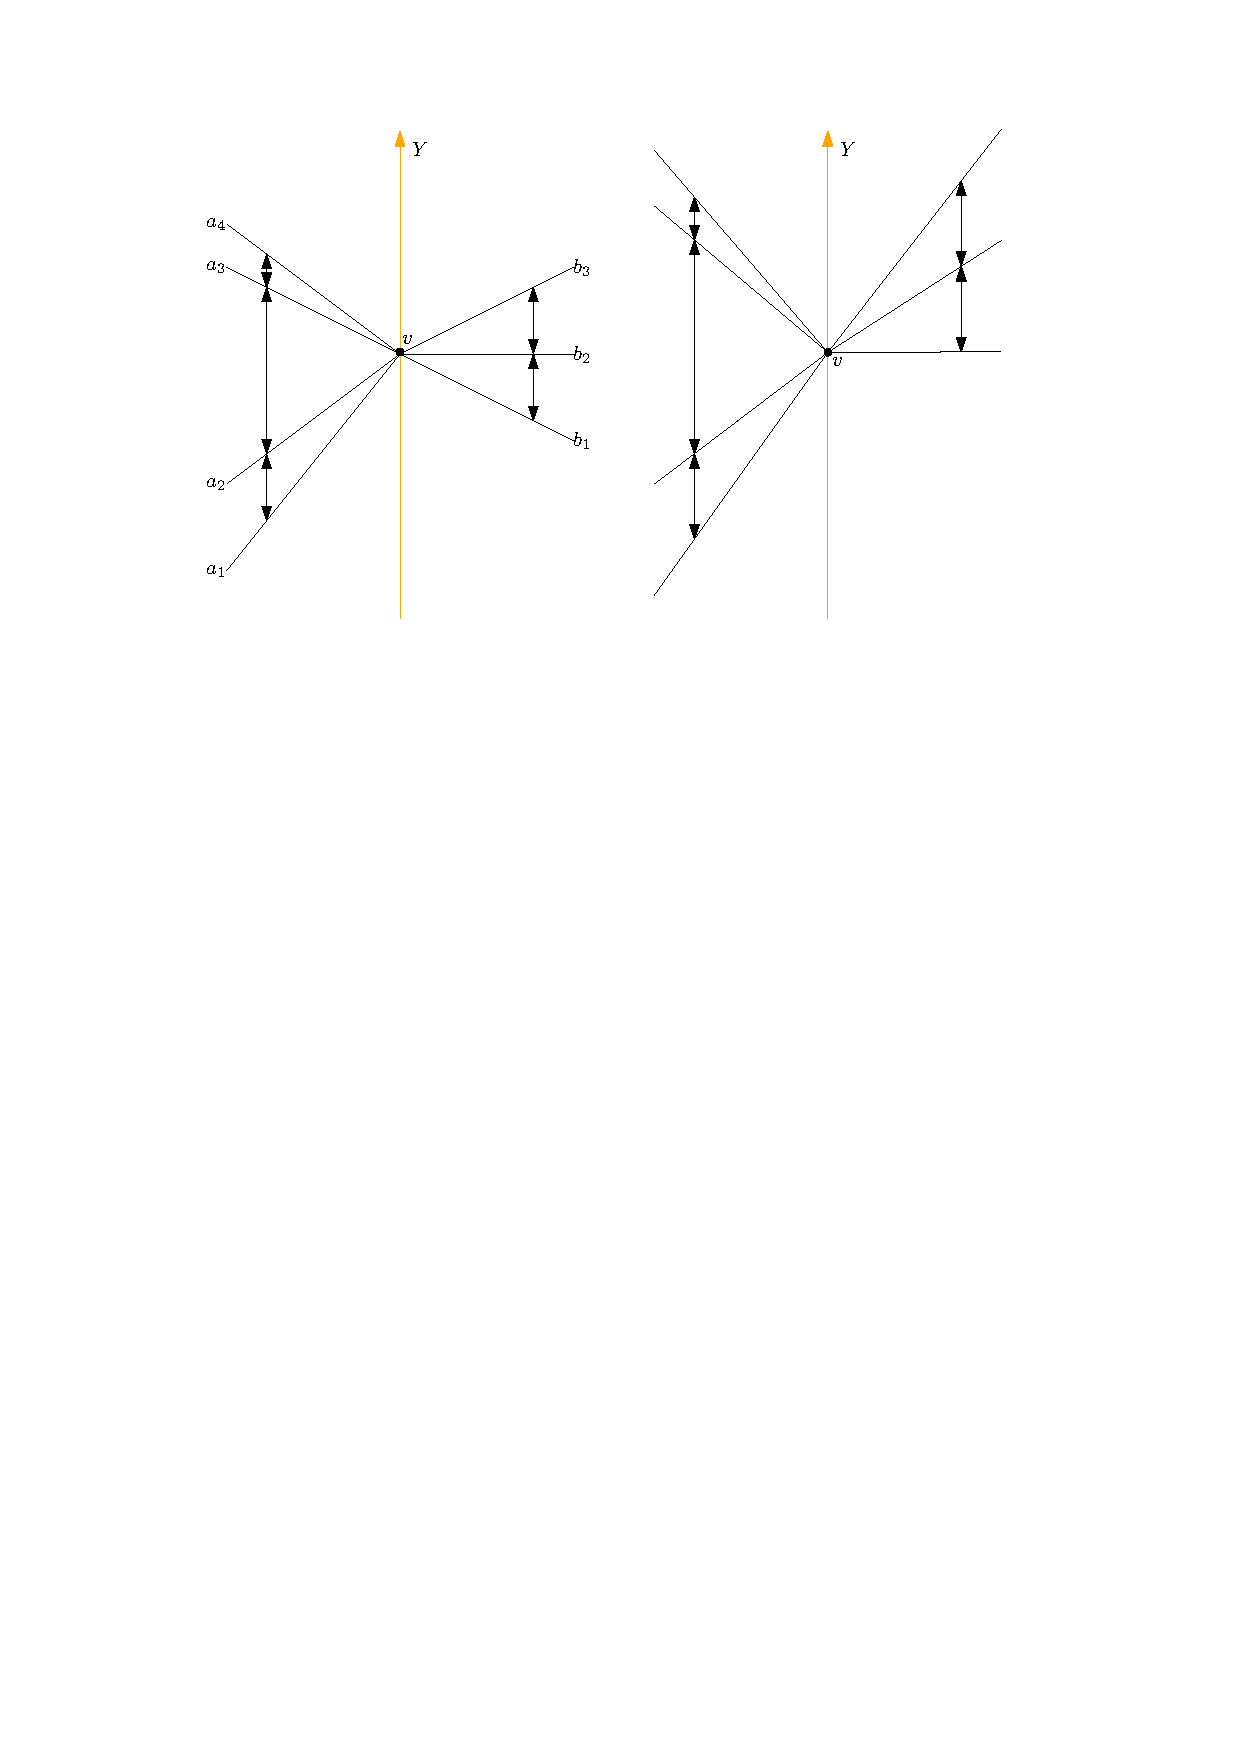
\includegraphics{figs/proportional}}
%	\caption{The degrees of freedom provided by the proportionality constraints}
%	\figlabel{proportional}
%\end{figure}
\begin{lem} \label{le:number-of-equations}
The total number of equations \thetag{\ref{eq:slope0}},~\thetag{\ref{eq:proportion}}, and~\thetag{\ref{eq:proportion2}} is $m-4$.
\end{lem} 

To achieve the desired number, $m$, of equations, we add
four \emph{boundary equations}.  If the outer face is a quadrilateral, we set
the slopes $s_1$, $s_a$, $s_b$, and $s_m$ of its edges $e_1$, $e_a$, $e_b$, and $e_m$ to the fixed values of the slopes of the edges of $\Delta$. If the outer face is a triangle $\alpha\beta\gamma$, with $\gamma\in Y$, we set the slopes $s_1$, $s_a$, and $s_m$ of the boundary edges $e_1$, $e_a$, and $e_m$ to the fixed values of the slopes of the edges of $\Delta$ and we pick another (non-boundary) edge $e_b$ incident to $\gamma$ and set its slope $s_b$ to a fixed value; this value is such that $s_b$ is either larger than each of $s_1$, $s_a$, and $s_m$ or smaller than each of $s_1$, $s_a$, and $s_m$, depending on whether the slope of $e_b$ in $G$ is larger than the slope of each of $e_1$, $e_a$, and $e_m$ or smaller than the slope of each of $e_1$, $e_a$, and $e_m$. Observe that no other cases are possible. Together with the proportionality constraints, this effectively pins all the slopes incident to $\gamma$ to fixed values.

Altogether, we have now a system of $m$ linear equations
in the $m$ unknowns $s=(s_1,\ldots,s_m)$, which we can write
compactly as
$A\cdot s = b$, with a square matrix $A$ whose entries come from
\thetag{\ref{eq:slope0}--\ref{eq:proportion2}}.
%are the variables we wish to solve for, and $b$ is a column $m$-vector
%whose entries also come from \eqref{slope}.  
Only four entries of
the right-hand side vector
$b$
are non-zero, due to the four boundary equations.
We will show that $A\cdot s=b$ has a unique
solution and that this solution gives a \Fary\ embedding of $G$.

\subsubsection{Setting Proportionality Constraints.}
%
%Since our plan is to show how to morph the given embedding of $G$ into the desired embedding, it is important that the given embedding satisfy the appropriate system of equations.  
%
We now specify how the coefficients in the proportionality constraints
are chosen, so that they are satisfied by the initial embedding.  The statement of \thmref{a-graph} assumes that $G$ is a \Fary\ embedding.  In this embedding, every edge $e$ intersects $Y$
in a single point $(0,y_e')$ and has a slope $s_e'$.  For a particular
vertex $v\in Y$, incident to edges $a_1,\ldots,a_k$ and $b_1,\ldots,b_\ell$
as described above, we use the slopes in the given embedding to set the
coefficients in the proportionality constraints.  In the notation used
in \eqref{proportion}, we set
$\lambda_i = (s_{b_i}'-s_{b_1}')/(s_{b_\ell}'-s_{b_1}')$
and in \eqref{proportion2}, we set $\mu = (s_{a_1}'-s_{a_k}')/(s_{b_\ell}'-s_{b_1}')$. This ensures that the slopes $s_{e_1}',\ldots,s_{e_m}'$ satisfy the
proportionality constraints.


\subsubsection{Ordering constraints.}
%
We define a relation $\prec$ on the edges of $G$, where $e_1 \prec e_2$ if and only if (1) $y_{e_1} < y_{e_2}$ and $e_1$ and $e_2$ have a common endpoint $v\in L$; or (2) $y_{e_1} > y_{e_2}$ and $e_1$ and $e_2$ have a common endpoint $v\in R$.
We say that a vector $s=(s_1,\ldots,s_m)$ \emph{satisfies the ordering
	constraints} if $s_{e_1} < s_{e_2}$ for every pair $e_1,e_2\in E(G)$
such that $e_1\prec e_2$. This definition captures the condition that vertices of $G$ in $L$ (respectively, $R$) should be embedded so that they remain in $L$ (respectively, $R$), as in the following. 

\begin{obs}\obslabel{left-right}
If a solution $s$ to $A\cdot s=b$ satisfies the ordering constraints, then every vertex that is in $L$ (in $R$) in $G$ is also in $L$ (respectively in $R$) in the embedding corresponding to $s$. 
\end{obs}

\begin{proof}	  
Consider any vertex $v$ that is in $L$ in $G$ and that is incident to (at least) two edges $e_1$ and $e_2$. Assume w.l.o.g.\ that $y_{e_1} < y_{e_2}$, and hence that $e_1 \prec e_2$. Since $s$ satisfies the ordering constraints we have $s_{e_1} < s_{e_2}$, hence the lines with slopes $s_{e_1}$ and $s_{e_2}$ through $(0,y_{e_1})$ and $(0,y_{e_2})$, respectively, meet in $L$. The argument for the vertices in $R$ is analogous. 
\end{proof}	  

Note that $\prec$ is acyclic since $G$ is an A-graph and therefore the slopes $s_{e_1}',\ldots,s_{e_m}'$ of edges
in $G$ satisfy the ordering constraints.  This would not be possible if $\prec$ contained cycles. 
%  Indeed, $i_1\prec
% \cdots \prec i_r$ implies that, for each $j\in\{3,\ldots,r\}$, $y_{i_j}\in
% (\min\{y_{i_{j-1}},y_{i_{j-2}}\}, \max\{y_{i_{j-1}},y_{i_{j-2}}\})$. Thus,
% a chain in $\prec$ corresponds to a sequence of strictly nested intervals.

\begin{lem}\lemlabel{order-gives-embedding}
	Any solution $s$ to $A\cdot s=b$ satisfying
	the ordering constraints % $\prec$
	yields a
	\Fary\ embedding of $G$.
\end{lem}

\begin{proofsketch}
Devillers \etal\ \cite{devillers.liotta.ea:checking} proved that a straight-line embedding $G'$ of a 2-connected graph $G$ is a \Fary\ embedding if: (i) for every vertex~$v$, the clockwise order of the edges around $v$ in $G'$ is the same as in $G$; and (ii) every face of $G$ is embedded without crossings in $G'$. In our case $G'$ is a straight-line embedding of $G$ given by a solution to $A\cdot s = b$ satisfying the ordering constraints. We prove that $G'$ satisfies conditions (i) and (ii) by using \obsref{left-right} and the fact that the slopes of the edges of $G'$ satisfy equations~\eqref{slope0}--(\ref{eq:proportion2}); in particular, for a vertex $v\in Y$, it is ruled out that the clockwise order of the edges around $v$ in $G'$ is reversed with respect to $G$ by the ordering constraints for the vertices of the triangles incident to $v$.
\end{proofsketch}


Any solution $s$ to $A\cdot s=b$ has the outer face drawn as $\Delta$, by the boundary constraints, and has the intersection between $e_i$ and $Y$ at $(0,y_i)$, by the concurrency constraints. Hence, by~\lemref{order-gives-embedding} ensuring the existence of a solution $s$ to $A\cdot s=b$ satisfying the ordering constraints is enough to prove~\thmref{a-graph}.

\subsubsection{Strong Ordering Constraints.}
\label{strong}
%
For some $\epsilon \ge 0$, we say that $s=(s_1,\ldots,s_m)$ satisfies
the \emph{$\epsilon$-strong ordering constraints} if, for each
$i,j\in\{1,\ldots,m\}$ such that $e_i\prec e_j$, the inequality
$s_j-s_i > \epsilon$ holds.
% A solution $s$ that satisfies
Clearly, any $s$ satisfying the $\epsilon$-strong ordering constraints also satisfies the ordering constraints. The converse holds when equations~\thetag{\ref{eq:slope0}}--\thetag{\ref{eq:proportion2}} are satisfied, for a suitably small $\epsilon$, as in the following.

\begin{lem}\lemlabel{weak-to-strong}
	Any solution $s$ to $A\cdot s=b$ that satisfies
	the ordering constraints
	also satisfies 
	the $\epsilon$-strong ordering constraints
	for all $\epsilon<\min\{|y_i-y_j| : 1\le i< j\le m\}$.
\end{lem}

\begin{proof}
	By \lemref{order-gives-embedding} every vertex is contained in the interior or on the boundary of $\Delta\subset[-1,1]^2$.
	Hence, every $x$-coordinate is
	in the interval $[-1,1]$.
	A vertex incident to $e_i$ and $e_j$ has $x$-coordinate
	$(y_j-y_i)/(s_i-s_j)$.
	From $|(y_j-y_i)/(s_i-s_j)|\le 1$ we derive
	$|s_i-s_j|\ge|y_j-y_i| > \epsilon$.
\end{proof}

\subsubsection{Uniqueness of Solutions Satisfying Ordering Constraints.}
%
The utility of the $\epsilon$-strong ordering constraints is that they
allow us to appeal to continuity. 
%It is impossible 
%to violate
%the ordering constraints without first violating the
%$\epsilon$-strong ordering constraints.
%But since the ordering constraints imply the
%$\epsilon$-strong ordering constraints,
%it is not possible
%to violate
%the ordering constraints at all.
% by showing that, if $A\cdot s=b$
%were to have some undesireable property, then some function which we
%know to be continuous would have a discontinuity.
An example will be seen in the following proof.

\begin{lem}\lemlabel{unique}
	If $s$ is a solution to $A\cdot s=b$ that satisfies the ordering
	constraints, % $\prec$, 
	then $s$ is 
	the unique solution to $A\cdot s=b$.
\end{lem}

\begin{proof}
	Assume that $\epsilon$ is fixed so that $0<\epsilon<\min\{|y_i-y_j| : 1\le i< j\le m\}$.
	
	Suppose, for a contradiction, that there is a solution $s$ to $A\cdot s=b$ that satisfies the ordering
	constraints, % $\prec$,
	but is not unique.  Since $A\cdot s=b$ is a linear system, there is an entire (at least) 1-parameter family of solutions,
	i.e., there is a non-zero $m$-vector $r$ such that, for every
	$\lambda\in\mathbb R$, $A(s+\lambda r)=b$.
	
	
	Define the continuous (in fact, piecewise linear) function $f(\lambda) := \min \{\, (s_j+\lambda r_j)-(s_i+\lambda r_i) : e_i \prec
	e_j\,\}$ and let $\lambda^*$ be the value with the smallest absolute value
	$|\lambda^*|$ such that
	$f(\lambda^*)\le\epsilon/2$. 
	
	In order to prove that $\lambda^*$ exists, it suffices to prove that a value $\lambda$ exists such that $f(\lambda)\le 0$. Note that $r_1=r_a=r_b=r_m=0$ since the slopes $s_1$, $s_a$, $s_b$, and $s_m$
	are fixed.
	Since $G$ is connected and $m\geq 5$, there is at least one vertex $v$ with two incident edges $e_k$
	and $e_\ell$ such that $r_k=0$ and $r_\ell\neq 0$. 
	We can thus pick $\lambda$ so that $(s_\ell+\lambda r_\ell)-(s_k+\lambda r_k)=s_\ell-s_k+\lambda r_\ell=0$,
	and then $f(\lambda)\le 0$. Hence $\lambda^*$ exists.
	
	Now we know that, for any $\lambda$ between $0$ and $\lambda^*$ and for any $i$ and $j$ such that $e_i\prec e_j$, the difference $(s_j+\lambda r_j)-(s_i+\lambda r_i)$ has the same sign as $s_j-s_i$. It follows that the slopes satisfy the ordering constraints throughout
	this interval, and
	\lemref{weak-to-strong} implies that $f(\lambda^*)\ge\epsilon$, a contradiction.
\end{proof}

%The proof of \lemref{unique} was quite explicit (perhaps overly so)
%in showing the discontinuity caused by the $\epsilon$-strong ordering
%constraints.  In subsequent arguments we will not be quite so explicit.

\subsubsection{A Parametric Family of Linear Systems.}
%
Note that $A$ and $b$ are functions of $y=(y_1,\ldots,y_m)$ and of the
four slopes $h=(s_1,s_a,s_b,s_m)$. We make this explicit, by writing
$A_1=A(y,h)$ and $b_1=b(y,h)$.

Let $y'=(y_1',\ldots,y_m')$ and $s'=(s_1',\ldots,s_m')$ denote the
$y$-intercepts and the slopes of the edges in the initial embedding of $G$
and let $h'=(s_1',s_a',s_b's_m')$. 

Consider the system $A(y',h')\cdot s = b(y',h')$.  This system has
at least one solution $s=s'$.  We now define
a continuous family of linear systems that interpolates between $A(y',h')\cdot s=b(y',h')$ and $A(y,h)\cdot s=b(y,h)$. Suppose first that the outer face of $G$ is delimited by a quadrilateral.

For $0\le t\le 1$ and $i\in\{1,a,b,m\}$,  define $s_i(t)=(1-t)s_i' + ts_i$ and $h(t)=(s_1(t),s_a(t),s_b(t),s_m(t))$.
Note that $s_1(t)-s_a(t) = (1-t)(s_1'-s_a') + t(s_1-s_a) > 0$. Inequalities $s_1'-s_a'>0$ and $s_1-s_a>0$ come from the assumption that the vertex incident to  $e_1$ and $e_m$ is in $L$ both in $G$ and in $\Delta$. Similarly, we have $s_m(t)-s_1(t)>0$ and $s_b(t)-s_m(t)>0$. Then we can define $\epsilon_1 = \min_{0\le t\le 1}\min\{s_1(t)-s_a(t), s_m(t)-s_1(t), s_b(t)-s_m(t)\}$ and observe that $\epsilon_1>0$. Analogously, for $0\le t\le 1$ and $i\in\{1,\ldots,m\}$, define $y_i(t) = (1-t)y_i' + ty_i$ and  $y(t)=(y_1(t),\ldots,y_m(t))$.
Note that, for any
$1\le i< j\le m$ and any $0\le t\le 1$, we have $y_j(t) - y_i(t) = (1-t)(y'_j-y'_i) + t(y_j-y_i) > 0$. Let $\epsilon_2=\min_{0\le t\le 1}\min\{y_j(t)-y_i(t): 1\le i< j\le m\}$ and observe that $\epsilon_2 >0$.  

  
%denominators in \eqref{slope} have absolute values bounded from below
%by $\epsilon_2$.  Thus, each entry in $A_t$ and $b_t$ is finite and is a
%uniformly continuous function of $t$.  

The entries in $A_t$ and $b_t$ are obtained in the same way as the entries of $A$ and $b$ were derived earlier, however each entry is now a linear function of~$t$, as $y$ and $h$ are replaced by $y(t)$ and $h(t)$, respectively, in the determination of the equations represented by $A_t$ and $b_t$.
Consider the unique quadrilateral $\Delta(t)$ whose edges cross $Y$ at
$y_1(t)$, $y_a(t)$, $y_b(t)$, $y_m(t)$ and have slopes $s_1(t)$,
$s_a(t)$, $s_b(t)$, and $s_m(t)$, respectively. Note that $\Delta(0)$ is the quadrilateral delimiting the outer face of $G$, while $\Delta(1)=\Delta$. Since $y_1(t),y_a(t),y_b(t),y_m(t)\in [-1,1]$, and since each of $s_1(t)$,
$s_a(t)$, $s_b(t)$, and $s_m(t)$ is at least $\epsilon_1$, we have that $\Delta(t)\subset[-1/\epsilon_1,1/\epsilon_1]\times[-\infty,\infty]$.
Hence, after scaling the $x$-coordinates by $1/\epsilon_1$,
\lemref{weak-to-strong} applies to $A_t\cdot s =b_t$, so any solution $s$
that satisfies $\prec$ also satisfies the $\epsilon^*$-strong ordering
constraints, for $\epsilon^*=\epsilon_1\cdot\epsilon_2$.

If the outer face of $G$ is delimited by a triangle, the arguments are analogous, however the inequalities $s_1(t)-s_a(t)>0$ and $s_m(t)-s_1(t)>0$ become either $s_m(t)-s_1(t)>0$ and $s_a(t)-s_m(t)>0$ or $s_1(t)-s_m(t)>0$ and $s_a(t)-s_1(t)>0$, depending on whether $(0,y_1)$ or $(0,y_m)$ is a vertex of $G$, respectively. Further, the inequality involving $s_b(t)$ now states  either $s_b(t)-s_a(t)>0$ or that $s_b(t)$ is smaller than the smallest between $s_1(t)$ and $s_m(t)$, depending on which of the two holds in $G$ (as when determining the boundary equations).

\subsubsection{Existence (and uniqueness) of solutions to $A_t\cdot s=b_t$.}
%
We now prove the following lemma which, together with \lemref{order-gives-embedding}, completes the proof of \thmref{a-graph}.

\begin{lem}\lemlabel{uniqueness}
	For every $0\le t\le 1$, the system $A_t\cdot s=b_t$ has a unique solution,
	and this solution satisfies the ordering constraints. % $\prec$.
\end{lem}

\begin{proof}
	Since $A_t$ is an $m\times m$ matrix, the system $A_t\cdot
	s=b_t$ has a unique solution~$s$ if and only if $\det A_t \neq 0$.
	When $\det A_t =0$, the system may have no solutions or
	multiple solutions.  
	When $\det A_t\neq 0$, 
	Cramer's Rule states that
	the solution
	is $s(t)=(s_1(t),\ldots,s_m(t))$ where, for each
	$i\in\{1,\ldots,m\}$, $s_i(t) = \frac{\det A_t^i}{\det A_t }$,
	and $A_t^i$ denotes the matrix $A_t$ with its $i$-th column replaced
	by $b_t$. 
	The numerators $\det A_t^i$ and the common
	denominator $\det A_t $ are polynomials in $t$, and therefore
	continuous
	functions of $t$.
	The solution $s(t)=(s_1(t),\ldots,s_m(t))$ depends continuously on $t$
	as long as  $\det A_t\ne0 $.
	
	
	We know that $A_0\cdot s=b_0$ has a solution $s'$ that satisfies the ordering constraints. By \lemref{unique}, this solution is unique, so $\det A_0\neq 0$.
	%
	Let $t^*:=\min \{t>0 :\det A_{t}= 0\}$. If $t^*$ does not exist we set $t^*=\infty$.
	% or $t>1$, we are
	% done.
	
	First we argue that, for $0\le t <\min \{1,t^*\}$, the unique solution $s(t)$ to $A_t\cdot s=b_t$ satisfies the ordering constraints. This argument is similar to the proof of \lemref{unique}. Suppose, for a contradiction, that a value $0<t<\min\{1,t^*\}$ exists for which $s(t)$ does not satisfy the ordering constraints. As $t$ increases its value from $0$ to $\min\{1,t^*\}$, since $s(t)$ depends continuously on $t$, a value is reached in which $s(t)$ violates the $\epsilon^*$-strong ordering constraints, while it does not violate the ordering constraints. This contradicts	\lemref{weak-to-strong}.
	
	If $t^*>1$ the same argument applies to $t=1$ and we are done.
	Assume, for a contradiction, that $0<t^*\le 1$.
	We look at whether the limit $s^*=\lim_{t\uparrow t^*}
	s(t)$ exists.
	Each function $s_i(t)$ is a quotient of two polynomials; thus, for $t\to t^*$ it can either converge to $s_i(t^*)$ continuously, or diverge to $+\infty$ or $-\infty$.
	%
	For $t<t^*$ all solutions $s(t)$ to the systems $A_t\cdot s=b_t$ satisfy the $\epsilon^*$-strong ordering constraints.
	Hence, if the limit exists, by continuity, it also satisfies $A_{t^*}\cdot s^*=b_{t^*}$
	and the $\epsilon^*$-strong ordering constraints.
	By \lemref{unique}, the solution $s^*$ is
	the unique solution
	of $A_{t^*}\cdot s=b_{t^*}$, which contradicts the assumption
	$\det A_{t^*}= 0$.
	
	The proof of the lemma is completed by ruling out the possibility that $A_{t^*}\cdot s=b_{t^*}$ has no solution because $\lim_{t\uparrow t^*} s(t)$ does not exist. This proof is deferred to the full version of the paper in the appendix. 
\end{proof}
